\documentclass{scrreprt}

%Für deutsche Trennung
\usepackage[ngerman]{babel}
%Für UTF8-Codierung, mit Umlauten!
\usepackage[utf8]{inputenc}

%Für Links, auch innerhalb des Dokuments
\usepackage{hyperref}

%Einbinden von Grafiken
\usepackage{graphicx}

\usepackage{booktabs}

% Zusatzpakete verbatim und moreverb: listing-Umgebung
\usepackage{verbatim, moreverb}
\usepackage{color}
\definecolor{darkred}{rgb}{0.5,0,0}
\usepackage{listings}		%Für Quellcode

\tolerance=1000

\lstloadlanguages{Java, XML}
\lstset{language=Java}
\lstset{
basicstyle=\ttfamily, % alle listings scriptsize drucken (kann man gerade noch lesen) und Schreibmaschinenschrift für alles
keywordstyle=\color{darkred}\bfseries, % Schlüsselwörter fett und dunkelrot drucken
commentstyle=\color{blue}, % Kommentare blau drucken
showstringspaces=false, % Strings im Code ohne Kenntlichmachung von Leerzeichen
breaklines=true,
frame=lines,
numbers=left,
numberstyle=\tiny,
tabsize=3
}

\newcommand{\lstx}[1]{\lstinline$#1$} 


\title{Software Quality Measurement}
\author{Gruppe H}
\date{\today}

\begin{document}

\maketitle
\tableofcontents

\chapter{Software Quality Measurement}

Für \lstx{mallet}\footnote{\href{https://github.com/mimno/Mallet}{Mallet af github}}, eine Verarbeitungssoftware für natürliche Sprache, sollen beispielhaft Kenngrößen für Softwarequalität ermittelt und ausgewertet werden. Zur Berechnung der Kenngrößen wird \lstx{ckjm}\footnote{\href{https://github.com/dspinellis/ckjm}{ckjm auf github},  \href{https://www.spinellis.gr/sw/ckjm/doc/indexw.html}{Manual}} verwendet, das alle sechs Kenngrößen (Metriken zum Messen von Softwarequalität) nach Chidamber and Kemerer sowie zwei zusätzliche ermittelt. Die Ausgaben von \lstx{ckjm} werden mit Hilfe eines zur Verfügung gestellten, auf \lstx{matplotlib} basierenden Pythonskripts aufbereitet und in Form von Histogrammen dargestellt.

\begin{lstlisting}[caption = Beispiele für den Output von mallet]
cc.mallet.extract.test.TestDocumentExtraction 7 0 0 20 31 21 0 7
cc.mallet.pipe.SerialPipes$Predicate 2 1 0 2 3 1 1 2
cc.mallet.classify.BalancedWinnowTrainer 6 0 0 11 21 11 1 6
cc.mallet.util.CharSequenceLexer 20 1 0 1 45 94 14 16
...
\end{lstlisting}


%TODO Output the 3 classes with the highest and lowest scores for the measures CBO and LCOM. (You may use the provided file findExtremes.py for doing this) Have a look at those classes, why do they have high/low scores for CBO and LCOM? How do you judge the quality of the classes and the effectiveness of the measures? Write a short explanation. 

\section{CBO - Kopplung ziwschen Objektklassen}
CBO 
CBO: Coupling between object classes

\begin{figure}
 \centering
 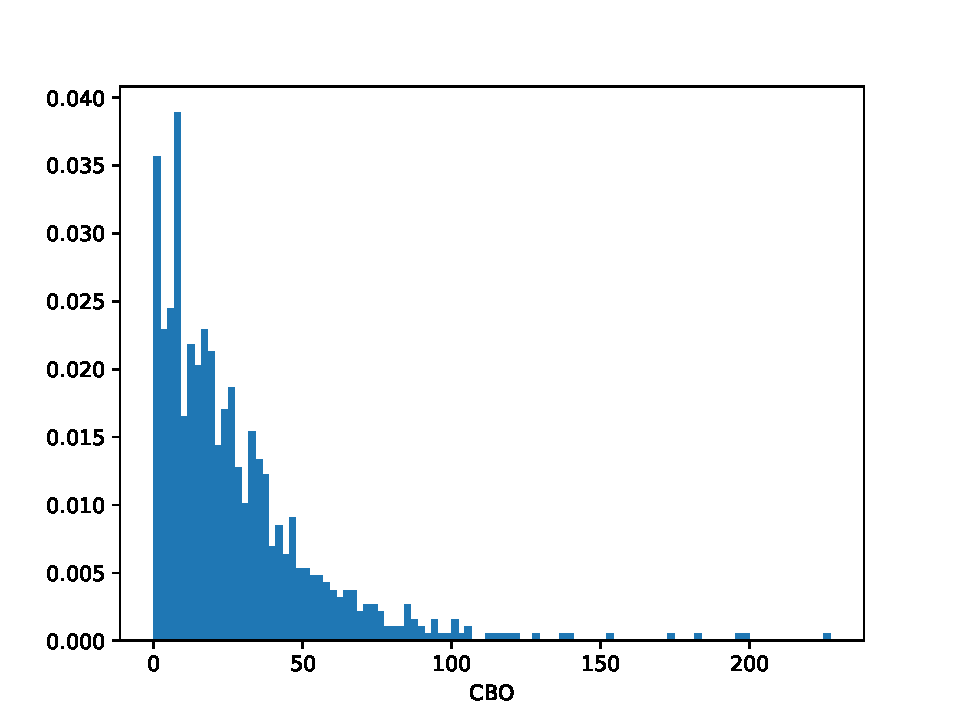
\includegraphics[width=.8\textwidth]{./CBO.pdf}
 % CBO.pdf: 0x0 pixel, 300dpi, 0.00x0.00 cm, bb=
 \caption{Coupling of Object Classes}
 \label{abb:cbo}
\end{figure}


\begin{center}
\begin{tabular}{ll}
\toprule
CBO: schlechteste Klassen\\
\midrule
\lstx{cc.mallet.optimize.OptimizerEvaluator} & 0\\
\lstx{cc.mallet.util.tests.TestAStar\$1} & 0\\
\lstx{cc.mallet.pipe.CharSequenceRemoveHTML\$1} & 0 \\
\bottomrule
\end{tabular}
\end{center}


\begin{center}
\begin{tabular}{ll}
\toprule
CBO: beste Klassen\\
\midrule
\lstx{cc.mallet.topics.ParallelTopicModel} & 227 \\
\lstx{cc.mallet.fst.tests.TestCRF} & 198\\
 \lstx{cc.mallet.topics.LDAHyper}&196 \\
\bottomrule
\end{tabular}
\end{center}


Ein hoher Wert des CBO ist erwünscht. Das bedeutet, dass Methoden mit vielen Instanzvariablen eng gekoppelt sind, was sich wiederum positiv auf die Softwarequalität auswirkt.

Ein kleiner Wert ist unerwünscht, da dies bedeutet, dass alle Methoden der Klasse eigene unabhängige Instanzvariablen benutzen. Dies wirkt sich negativ auf die Softwarequalität aus.

Das Histogramm zeigt die CBO-Werte aller getesteten Klassen. Die meisten CBO-Werte liegen im Bereich von 0 bis 50.

\section{LCOM - Mangel an Abgeschlossenheit}

LCOM: Lack of cohesion in methods

\begin{figure}
 \centering
 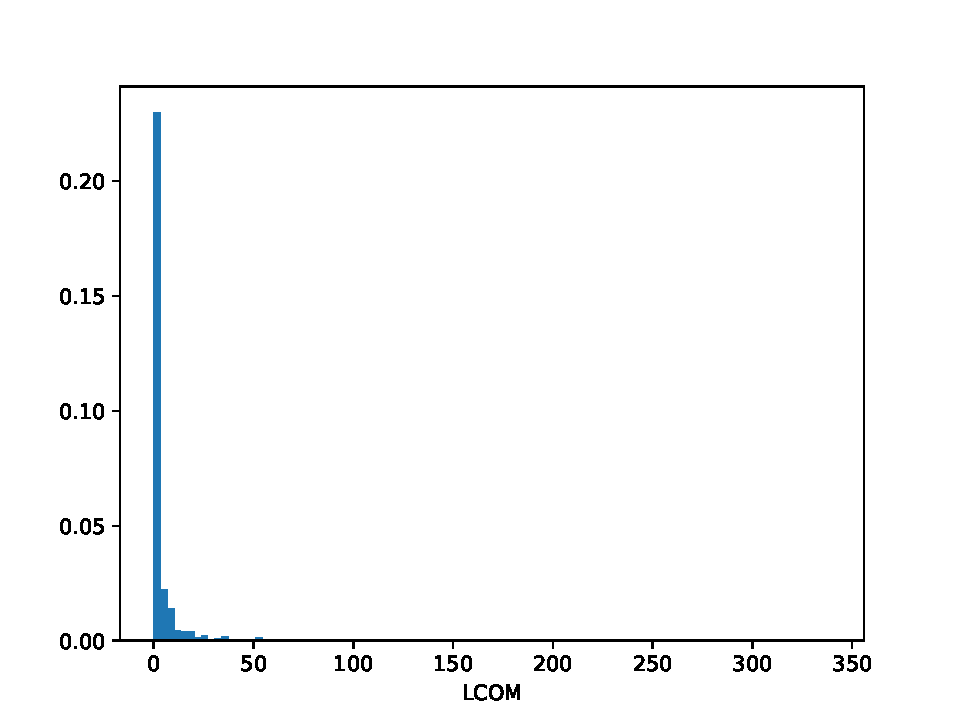
\includegraphics[width=.8\textwidth]{./LCOM.pdf}
 % LCOM.pdf: 0x0 pixel, 300dpi, 0.00x0.00 cm, bb=
 \caption{Lack of Cohesion}
 \label{abb:lcom}
\end{figure}


\begin{center}
\begin{tabular}{ll}
\toprule
LCOM: beste Klassen\\
\midrule
\lstx{cc.mallet.extract.test.TestDocumentExtraction} &0 \\
\lstx{cc.mallet.fst.LabelDistributionEvaluator} &0 \\
\lstx{cc.mallet.optimize.OptimizerEvaluator\$ByBatchGradient} &0  \\
\bottomrule
\end{tabular}
\end{center}


\begin{center}
\begin{tabular}{ll}
\toprule
LCOM: schlechteste Klassen \\
\midrule
\lstx{cc.mallet.pipe.Pipe} & 229\\
\lstx{cc.mallet.types.InstanceList} & 241\\
\lstx{cc.mallet.types.Instance} & 339 \\
\bottomrule
\end{tabular}
\end{center}

Im Vergleich zum CBO-Wert verhält sich der LCOM-Wert komplementär. Ein hoher Wert steht für den Mangel an Kohäsion (Zusammenhang zwischen den Methoden) und wirkt sich somit negativ auf die Softwarequalität aus.
Ein niedriger Wert bedeutet keinen Mangel und ist somit positiv für die Softwarequalität.

\pagebreak

\section{Weitere Kenngrößen und graphische Darstellung}

%TODO 7. Plot a histogram for each of the measures using matplotlib. (You may use the provided file findExtremes.py for doing this) What insights do you gain from these plots concerning the Mallet repository? You may compare the repository to other repositories of your choosing.

Die Kenngrößen werden als normierte Histogramme dargestellt, auf der x-Achse sind Bereiche möglicher Werte der Kenngröße aufgetragen. Auf der y-Achse der Anteil der Klassen, die diesem Wertebereich zugeordnet sind.

Als weitere Kenngrößen wurden von \lstx{ckjm} ermittelt:

\begin{itemize}
\item WMC: Weighted methods per class
    \begin{itemize}
    \item WMC betrachtet die Komplexität (Erweiterbarkeit und Verständlichkeit) der Klassen. Größere Werte sind negativ. Kleinere Werte sind positiv.
    \end{itemize}

\item DIT: Depth of Inheritance Tree
    \begin{itemize}
    \item DIT misst die Tiefe des Vererbungsbaums. Je tiefer dieser Baum ist, desto negativer wirkt sich das auf die Softwarequalität aus, weil es dann schwieriger ist, die Vererbungsstruktur bis in die Blätter nachzuvollziehen. D.h. in unserem Histogramm sind solche Klassen gut, die den Wert 0 haben, weil die Tiefe des Baums
    \end{itemize}

\item NOC: Number of Children
    \begin{itemize}
    \item NOC misst die Anzahl der Subklassen, die direkt unter der gemessenen Klasse existieren. Ein hoher Wert bedeutet, dass diese Klasse oft wiederverwendet wird und somit Code gesapart wird. Das bedeutet aber auch, dass eine Klasse mit hohem Wert gut getestet muss, um die Softwarequalität zu steigern. Im Vergleich zu DIT misst NOC die Breite des Baums, statt der Tiefe.
    \end{itemize}

\item RFC: Response for a Class
    \begin{itemize}
    \item Der RFC Wert steht für die Anzahl aller möglichen auszuführenden Methoden innerhalb der Klasse. Je höher der Wert, desto höher die Komplexität der Klasse. Also ist ein hoher Wert nicht erwünscht.
    \end{itemize}

\item Ca: Afferent coupling (not a C\&K metric)
    \begin{itemize}
    \item Der Ca Wert bestimmt die Anzahl der Packages, die von der Package dieser Klasse abhängen. Ein hoher Wert bedeutet eine hohe Verantwortung für diese Package und ist somit negativ behaftet. Da unsere Klassen größtenteils niedrigere Werte besitzen, ist dies positiv für die Softwarequalität.
    \end{itemize}

%TODO @Rebecca: Bitte nochmal bewerten, ob das so richtig ist.
\item NPM: Number of Public Methods for a class (not a C\&K metric)
    \begin{itemize}
    \item Der NPM Wert bestimmt die Anzahl der public methods innerhalb der Klasse. Ein hoher Wert bedeutet eine große Verantwortung und hohe Komplexität und ist daher für die Softwarequalität nicht von Vorteil.
    \end{itemize}

\end{itemize}

\begin{figure}
 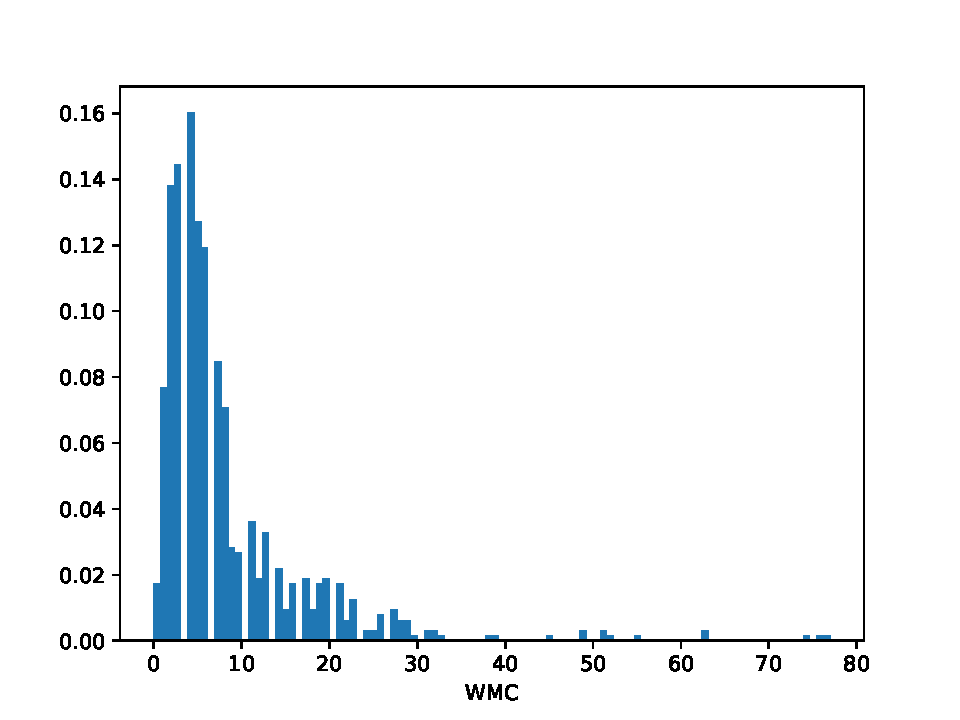
\includegraphics[width=.45\textwidth]{./WMC.pdf}
 % WMC.pdf: 0x0 pixel, 300dpi, 0.00x0.00 cm, bb=
  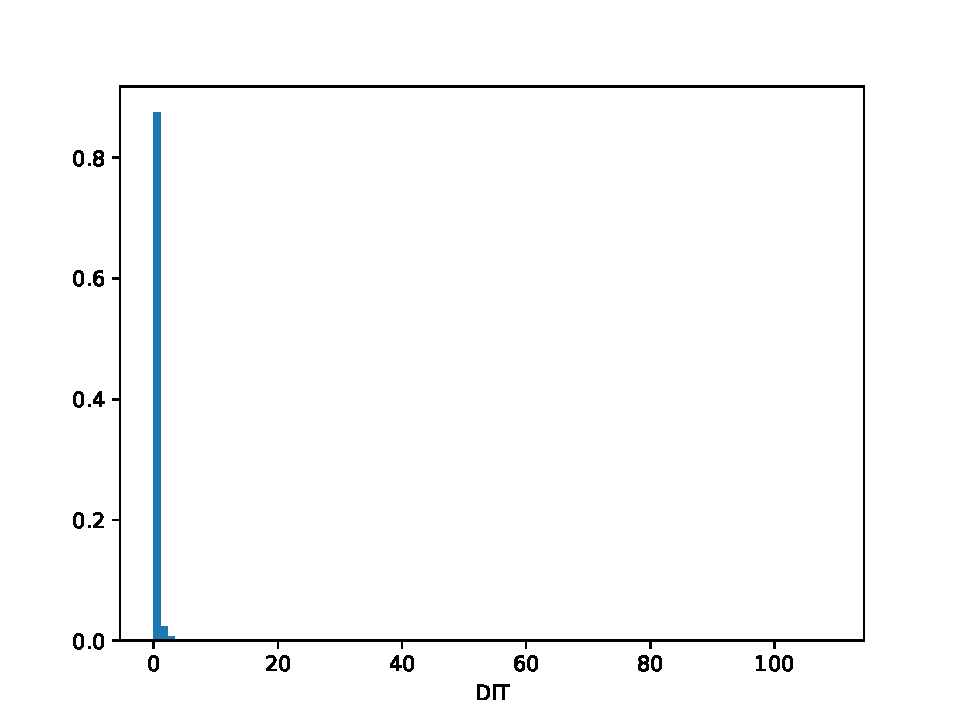
\includegraphics[width=.45\textwidth]{./DIT.pdf}
 \caption{WMC und DIT}
 \label{abb:wmc}
\end{figure}

% Depth of inheritance tree (DIT)
% This represents the number of discrete levels in the inheritance tree where
% subclasses inherit attributes and operations (methods) from superclasses. The
% deeper the inheritance tree, the more complex the design. Many object classes
% may have to be understood to understand the object classes at the leaves of the
% tree.

\begin{figure}
 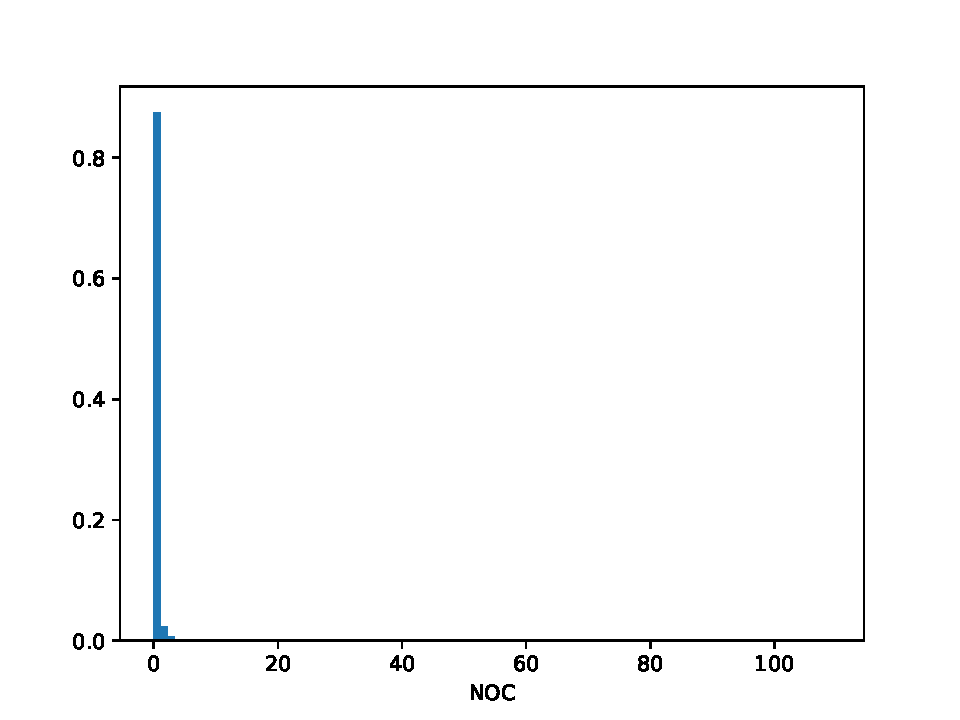
\includegraphics[width=.45\textwidth]{./NOC.pdf}
 % WMC.pdf: 0x0 pixel, 300dpi, 0.00x0.00 cm, bb=
  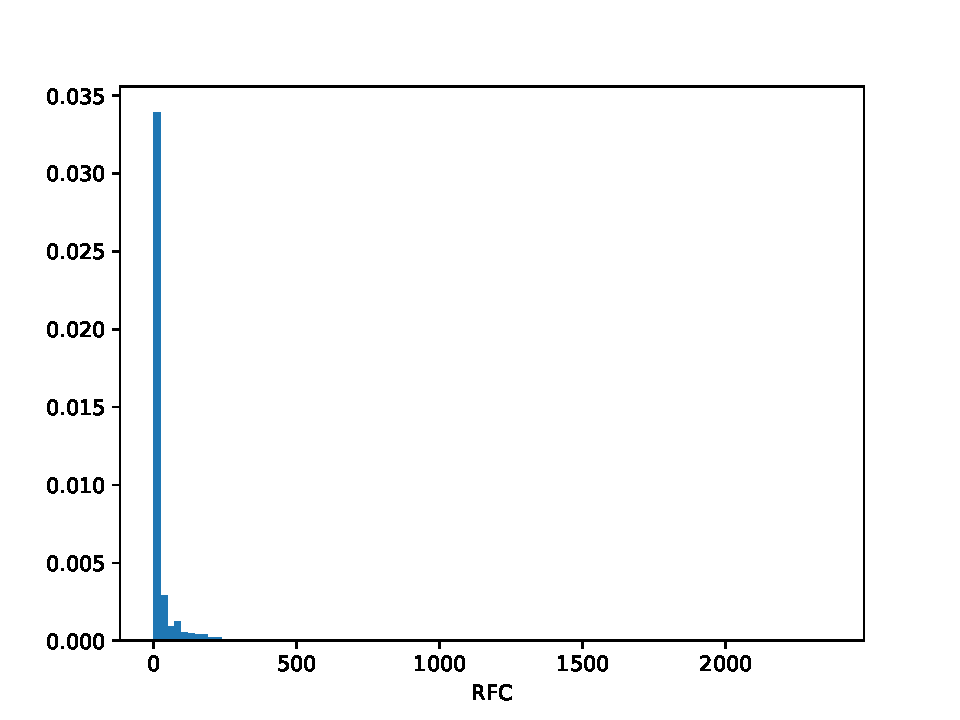
\includegraphics[width=.45\textwidth]{./RFC.pdf}
 \caption{NOC und RFC}
 \label{abb:noc_rfc}
\end{figure}

% Number of children (NOC)
% This is a measure of the number of immediate subclasses in a class. It measures
% the breadth of a class hierarchy, whereas DIT measures its depth. A high value
% for NOC may indicate greater reuse. It may mean that more effort should be
% made in validating base classes because of the number of subclasses that
% depend on them.

\begin{figure}
 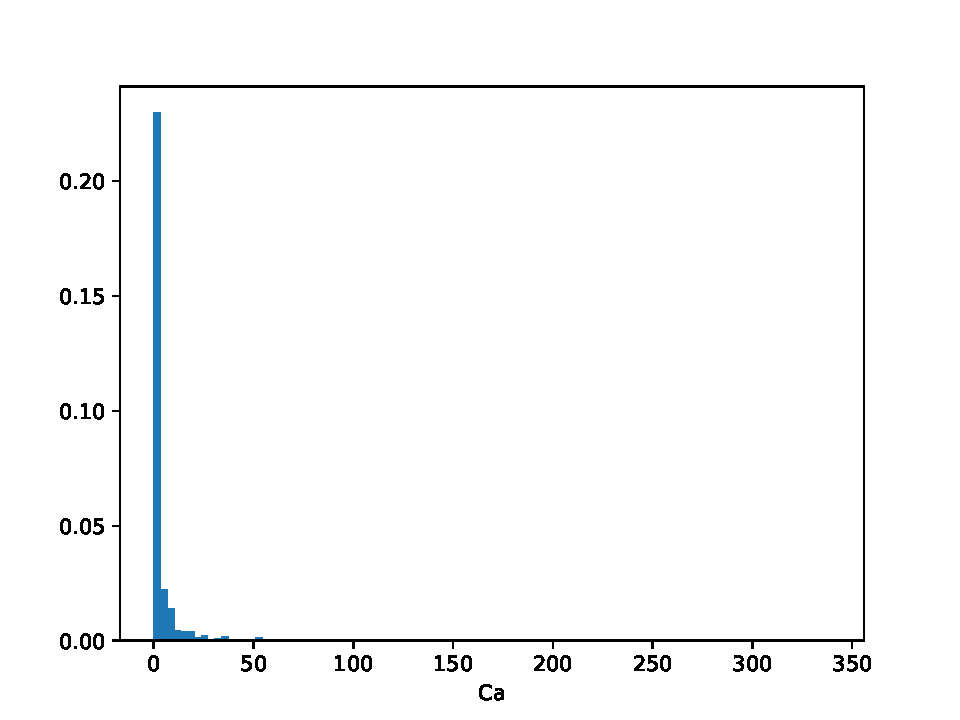
\includegraphics[width=.45\textwidth]{./Ca.pdf}
 % WMC.pdf: 0x0 pixel, 300dpi, 0.00x0.00 cm, bb=
  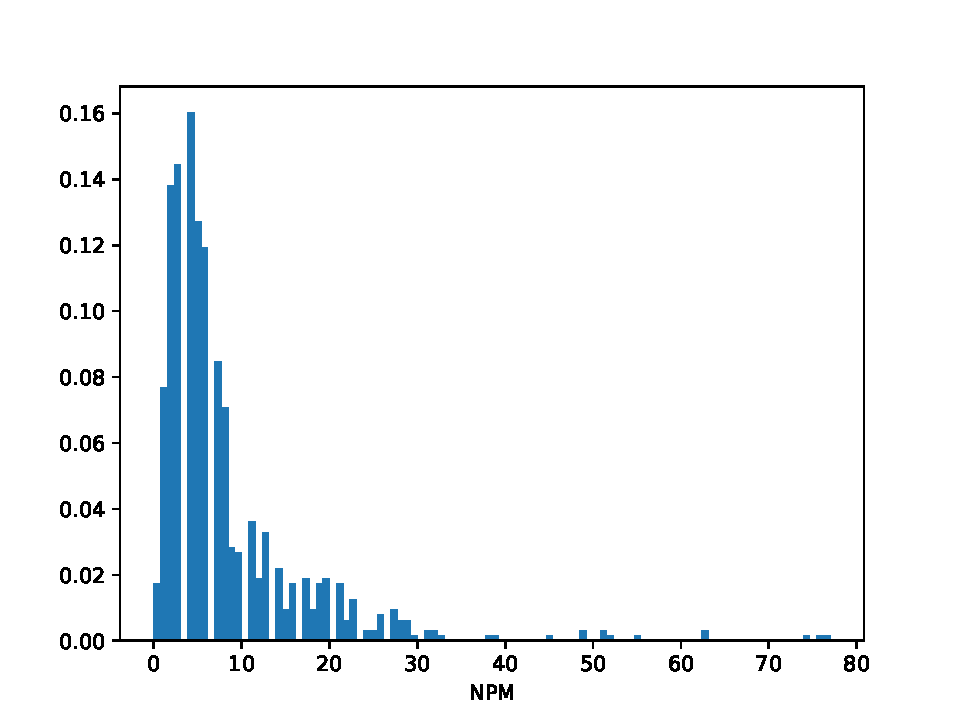
\includegraphics[width=.45\textwidth]{./NPM.pdf}
 \caption{Ca und NPM}
 \label{abb:ca_npm}
\end{figure}

\pagebreak

\section{Vergleich mit einer abgeänderten Version von mallet}

Dem Programm \lstx{mallet} werden zwei weitere Klassen \lstx{NewParallelTopicModel.java} und \lstx{TopicInferencerInterface.java} hinzugefügt. Nach dem Kompilieren wird die Analyse von \lstx{mallet} wiederholt und es werden die Kennzahlen der Klassen \lstx{NewParallelTopicModel} und \lstx{ParallelTopicModel} verglichen:

%TODO 8. In the package cc.mallet.topics there is a class called ParallelTopicModel which is used to learn a model on some data. A different class in the same package, called TopicInferencer, is used for the evaluation of the trained model. Add the provided Java files to this package and rebuild Mallet. Now compare the output of CKJM on ParallelTopicModel and NewParallelTopicModel. What do the new values indicate? What is the difference between the two classes?


\begin{tabular}{lllllllll}
\toprule
Klasse & WMC & DIT & NOC & CBO & RFC & LCOM & Ce & NPM \\
\midrule
\lstx{NewParallelTopicModel} & 68 & 1 & 0 & 22 & 233 & 800 & 0 & 61 \\
\lstx{ParallelTopicModel} & 63 & 1 & 2 & 21 & 227 & 627 & 11 & 58 \\
\bottomrule
\end{tabular}
%TODO Diese Tabelle muss noch beschrieben werden, ich hab keine Ahnung davon :/



\end{document}
